\subsection{机械振动}

\begin{tabularx}{\columnwidth}{XX}
  回复力      & $F=-kx$ \\
  简谐振动方程   & $x(t)=A\sin(\omega t+\varphi_0)$ \\
  速度与加速度   & $v=\omega A\cos(\omega t+\varphi_0)$，$a=-\omega^2x$ \\
  周期频率关系   & $T=\frac{2\pi}{\omega}$，$f=\frac{1}{T}$ \\
  弹簧振子周期   & $T=2\pi\sqrt{\frac{m}{k}}$\\
  单摆回复力    & $F=-\frac{mg}{l}x$ \\
  单摆周期     & $T=2\pi\sqrt{\frac{l}{g}}$ \\
  水平弹簧振子能量 & $E=\frac{1}{2}kx^2+\frac{1}{2}mv^2=\frac12kA^2$ \\
\end{tabularx}

\begin{formulanotebox}
\begin{itemize}[leftmargin=1.5em]
  \item 弹力和弹性势能相对于弹簧原长，振幅相对于平衡位置。
  \item 单摆周期公式适用于摆角较小的情形，且周期与摆球质量无关。
  \item 简谐运动中位移最大处速度为零、加速度最大；平衡位置处速度最大、加速度为零。
  \item 分离位置常见于弹簧原长、平衡位置或振幅位置，需结合约束判断。
  \item 振幅影响系统总能量，但需要满足题目给出的运动约束条件。
\end{itemize}
\end{formulanotebox}

\begin{keypointbox}
\begin{itemize}[leftmargin=1.5em]
  \item 判定简谐运动核心是“沿轨迹方向合力是否满足$F=-kx$”。
  \item 弹簧问题建议先画“原长-平衡-极值”三位置示意，再列能量关系。
\end{itemize}
\end{keypointbox}

\begin{center}
  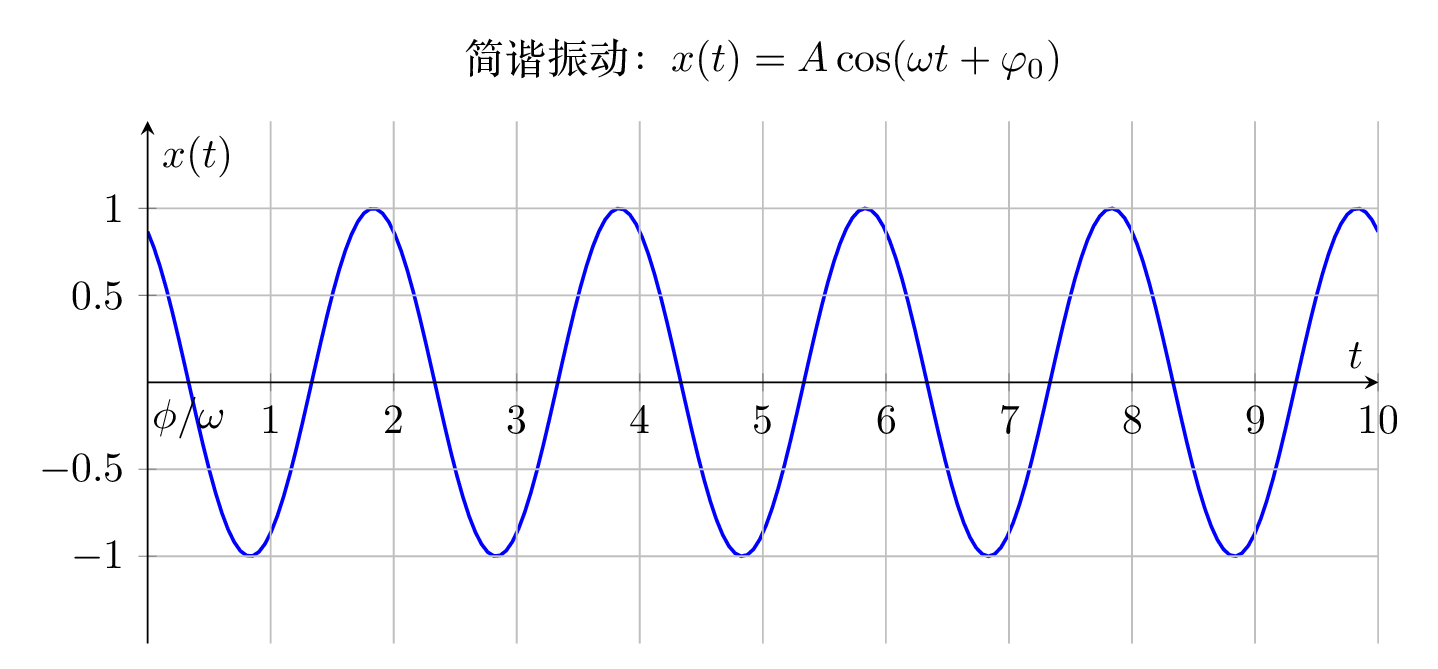
\includegraphics[width=0.72\columnwidth]{../assets/shm_vibration_equation.png}

  \vspace{4pt}
  {\small 简谐振动位移-时间图像示意}
\end{center}

\begin{center}
  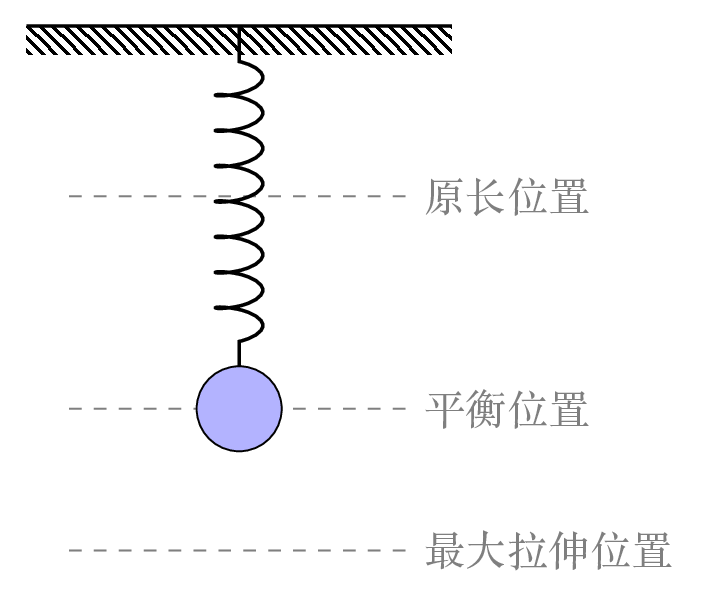
\includegraphics[width=0.62\columnwidth]{../assets/shm_spring_schematic.png}

  \vspace{4pt}
  {\small 弹簧振子原长/平衡/极值位置示意}
\end{center}

\begin{casetypebox}[title={\strut\textcolor{white}{\bfseries 常见题型：简谐振动判定}}]
\begin{itemize}[leftmargin=1.5em]
  \item 先找平衡位置，以偏离平衡位置的位移 $x$ 作为变量。
  \item 沿运动方向写合力，若能化成 $F=-kx$ 或 $a=-\omega^2x$，则为简谐运动。
  \item 图像题中，$x-t$ 图像读振幅和周期；斜率表示速度，曲线凹向反映加速度方向。
\end{itemize}
\end{casetypebox}

\begin{casetypebox}[title={\strut\textcolor{white}{\bfseries 常见题型：弹簧振子能量}}]
\begin{itemize}[leftmargin=1.5em]
  \item 水平弹簧振子常用 $\frac12kx^2+\frac12mv^2=\frac12kA^2$，其中 $x$ 是相对平衡位置的位移。
  \item 竖直弹簧振子可把重力影响并入新的平衡位置，围绕平衡位置仍满足简谐规律。
  \item 临界分离题要额外使用约束力为零的条件，不能只凭能量方程判断。
\end{itemize}
\end{casetypebox}
